\documentclass[twocolumns]{IEEEtran}
\usepackage{graphicx}
\usepackage{caption}
\usepackage{amsmath}
\usepackage{xcolor}

\graphicspath{{../figures/}}
\renewcommand\IEEEkeywordsname{Keywords}

\author{
	\IEEEauthorblockN{Erdal Sidal Dogan, Mert Komurcuoglu, Berkay Kurkcu} \\
	\IEEEauthorblockA{Facult of Engineering, MEF University \\
		Electrical \& Electronics Engineering Department}
}
\title{Audio Steganography}

\begin{document}
	\maketitle
	\begin{abstract}
		Digital Multimedia files such as images, videos, audio files etc. became ubiquitous in our lives. We can leverage these multimedia files for communication. Steganography is a technique for hiding information in these files in an imperceptible manner. By manipulating the multimedia signals, one can transmit messages to another in such a way that original signal would be indistinguishable from the manipulated one by a human. This paper demonstrates an application of audio steganography using MATLAB.
	\end{abstract}
	\begin{IEEEkeywords}
		Multimedia, steganography, signal.
	\end{IEEEkeywords}
	\section{Introduction}
	Steganography plays an important role in secret communication and data safety. There are many applications of steganography on different kinds of multimedia signals such as image, audio, video etc. along with multiple number of algorithms being used for similar purposes. In this project, we will be implementing the \textit{Least Significant Bit} algorithm on Audio signals using \textit{MATLAB}. Of course, there are multiple algorithms for similar purposes. However, after our researches we decided on LSB, since we don't need sophisticated needs such as fast encryption/decryption, higher amount of data transfer (bandwidth) etc, we considered the LSB would be an appropriate way to go. 
	
	
	\subsection{Literature Review}
	Data hiding in the least significant bits (LSBs) of
	audio samples in the time domain is one of the simplest
	algorithms with very high data rate of additional
	information . LSB coding  is one of the earliest
	techniques studied in the information hiding and
	watermarking area of digital audio (as well as other media
	types.  
	
	If we were to use more sophisticated methods we could use \textit{Threshold Based LSB} or \textit{Watermarking Method} algorithms. In \textit{Threshold Based LSB} method number of message bits changes depending on the amplitude of sampled signal\cite{threshold}. On the otherhand in \textit{Watermarking Method}, the LSB watermark encoder usually selects a subset and limits the number of of LSBs that can be imperceptibly modified during watermark embedding. The substitution operation on the LSBs is performed on this subset\cite{1286709}.
	
	
	Informations that we had from articles, we observed that,if
	16 bits per sample audio sequences are used,  the maximum LSB depth that
	can be used for LSB-based watermarking without causing
	noticeable perceptual distortion is the fourth LSB layer. According to the article, The tests
	were performed with a large collection of audio samples
	and individuals with different backgrounds and musical
	experience.
	
	\section{Method}
	\subsection{Embedding the Message to the Audio}
	Audio signals consist of thousands of samples which are represented as numerical values. As one can tell, all the numerical values are being stored in binary format by our computers. The binary format consist of 1's and 0's only. By looking at the positions of these 0 and 1's, we can get a decimal number. Right most digit of a binary number corresponds to $2^0$, as you move from right to left, power of 2 increases by 1. By adding the numbers shown as powers of 2 at where the bits on that position is 1, you can get a decimal number.
	\begin{figure}[h]
		\centering
		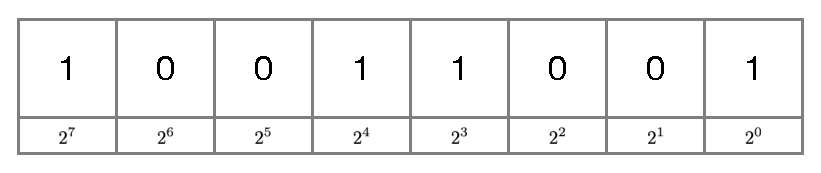
\includegraphics[scale=.5]{binary_num.eps}
		\caption{A binary number}
		\label{fig:binary}
	\end{figure}

	Figure \ref{fig:binary} shows the number $2^7 + 2^4 + 2^3 + 2^0 = 153$. As you can tell, the right-most bit of any binary number has a little effect on its decimal correspondent. For this example, if we flip the last bit from 1 to 0, decimal number would be equal to 152. Therefore, we can conclude that the right-most bit is the \textit{Least Significant Bit} of any binary number.
	
	The \textit{Least Significant Bit Algorithm} leverages this property of binary numbers for hiding messages in a audio file. As stated earlier, audio files consists samples that are represented by decimal number. Now, let's think about a sequence of an audio signal, assume it goes by; (normalized between -1 and 1)\\
	\begin{equation}
	\begin{bmatrix}
		0.143 & -0.471 & 0.643 & \hdots \\
	\end{bmatrix}
	\end{equation}
	The samples can be multiplied with a greater number to become integer values because the precision numbers representations are more complex than integer. Our input signal was decoded with 16 bits per sample. Thus, we multiplied each sample with $2^{15} = 32768$ for them to become integers that can be represented by 16 bits.
	\begin{equation}
		\begin{bmatrix}
		'000000000110010' \\
		'000000000000000' \\
		'000000000011001' \\
		'000000110100000' \\
		'000100100101011' \\
		'000010110101110' \\
		'001000110010010' \\
		\vdots
		\end{bmatrix} \\ \\		
	\end{equation}
	\begin{center}
		First 7 sample of an audio file
	\end{center}
	
	Now , let's focus on getting the binary representation of the message we want to embed into the audio file. We read this message from a .txt file, as a String, also, we add the symbol \ as an indicator of end of string. Similar to the audio files, the strings are also can be represented by integer values. As we know, a string is a sequence of characters, each character has a unique number assigned to it for computers to decode and display characters. Broadly used standard is ASCII. For this project we use ASCII standard also since MATLAB supports the decoding and encoding of ASCII represented values by default.
	\begin{figure}[h]
		\centering
		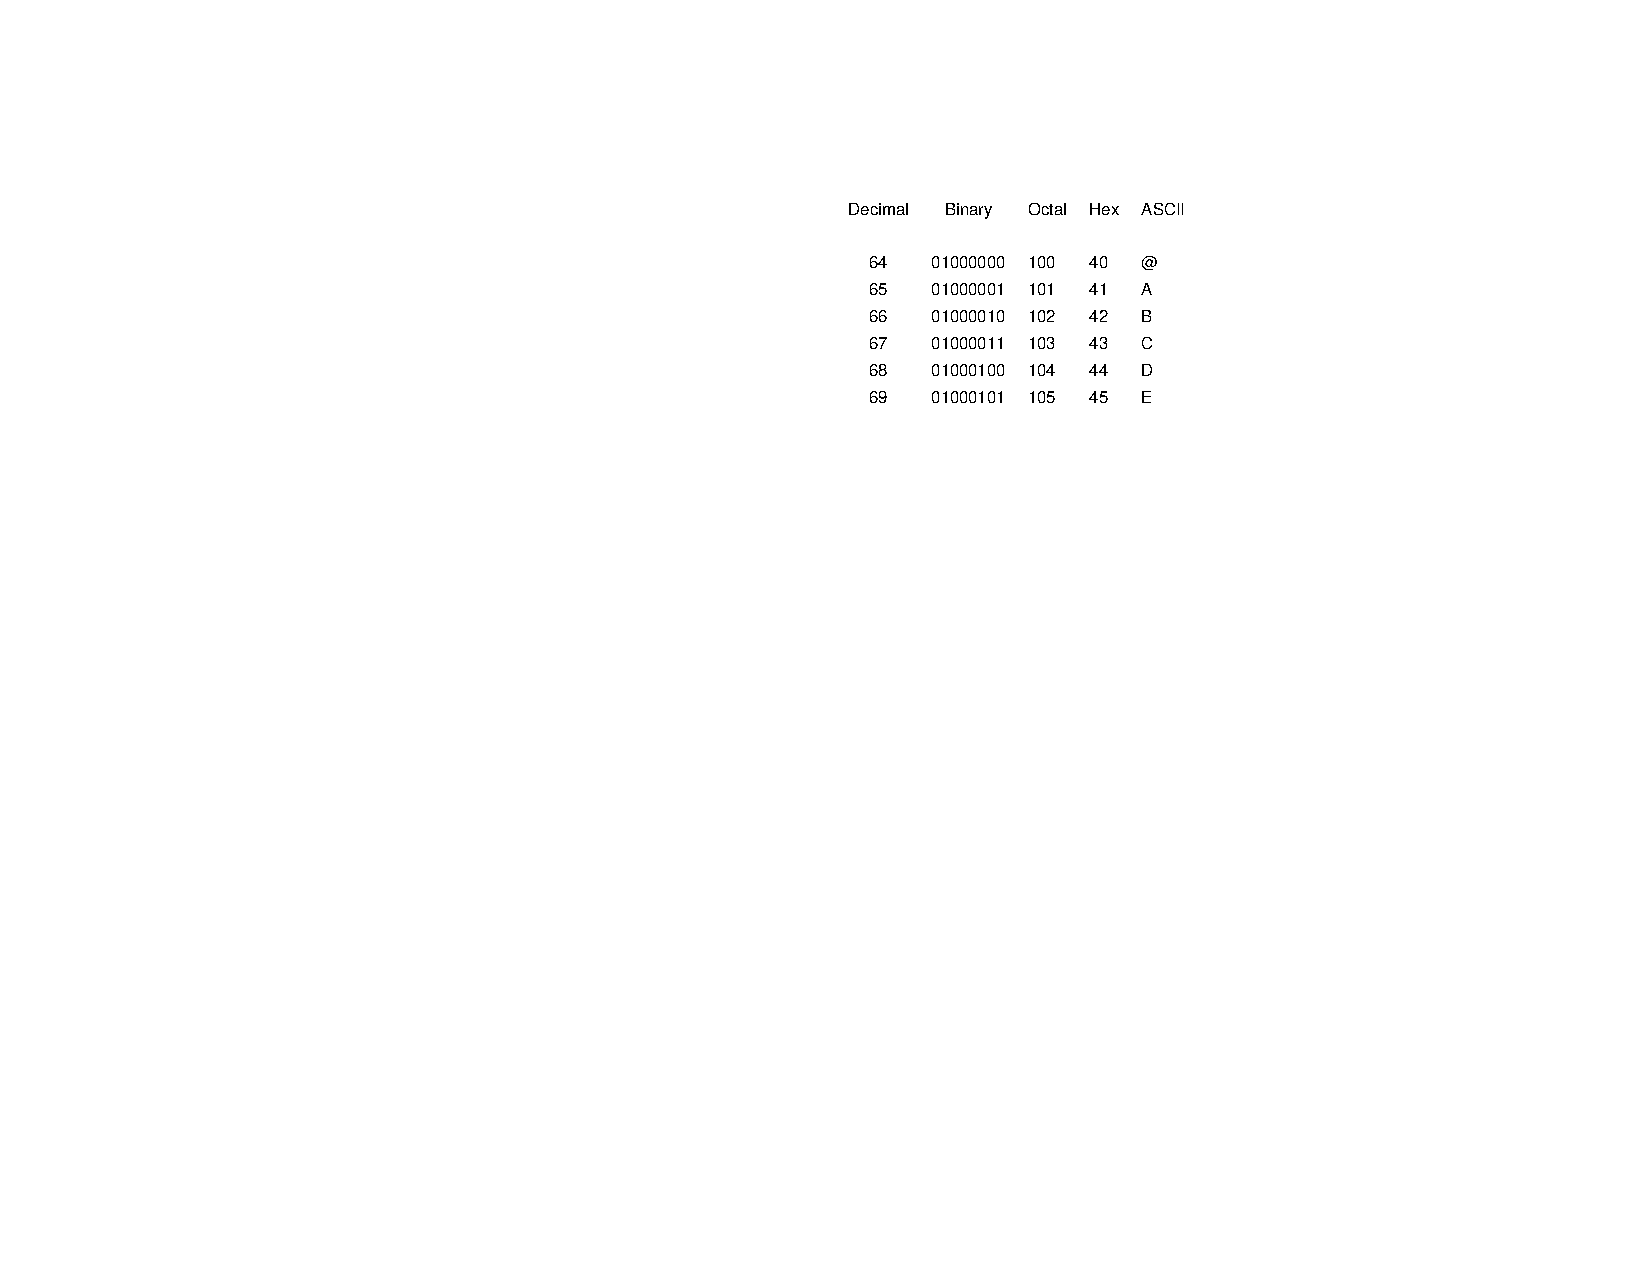
\includegraphics{ascii.pdf}
		\caption{ASCII codes of some characters}
	\end{figure}

	Let's start with the assumption of our text to be hidden being 
	\textbf{\texttt{Hello World!}}. First thing we do is to get the ASCII values of the characters. Then, we convert this integer numbers to their binary representations. When we do, we get an array of binary represented string, each item in the array corresponds to a character in the message.
	
	\begin{equation}
		\begin{bmatrix}
			\text{Binary} & \text{Decimal} & \text{Character} \\
			'1001000' & 72 & \text{H} \\
			'1100101' & 65 & \text{e}\\
			'1101100' & 108 & \text{l}\\
			'1101100' & 108 & \text{l}\\
			'1101111' & 157 & \text{o}\\
		\end{bmatrix} \\ \\		
	\end{equation}
	\begin{center}
		Binary representation of the word \textbf{\texttt{Hello}}
	\end{center}
	
	Having the binary representations of audio signal and the string itself, what we have to do is to embed the binary representations of string into the audio signal itself. As shown previously, right-most bit is the Least Significant Bit of a binary number, changing it doesn't change total value so much.
	
	We are going to iterate over the every bit of the binary representation of the string, and for every bit, we are going to change the least significant bit the binary representation of a sample from audio signal.
	
	\subsection{Extracting the message from the Audio}
	
	Extracting the message from an audio signal is exactly same as embedding it, but in reverse order. Of course we start by reading the audio signal in binary form. Then, we know that when we read last bits of each sample and group them by 8 bits, each group of 8 will correspond to a decimal number. Then, every decimal number will correspond to a unique character. By writing the characters we retrieved side by side, we get the string which was embedded to the audio file.
	
	\begin{equation}
			\begin{bmatrix}
				'00000000011001\color{red}1' \\
				'00000000000000\color{red}0' \\
				'00000000001100\color{red}0' \\
				'00000011010000\color{red}1' \\
				'00010010010101\color{red}0' \\
				'00001011010111\color{red}0' \\
				'00100011001001\color{red}0' \\
			\vdots
			\end{bmatrix} \\ \\		
		\end{equation}
	\begin{center}
		First 7 sample of an audio file which carries hidden information
	\end{center}
	If you compare the binary representation of letter \texttt{H} and the Least Significant Bits of the samples from the carrier file -highlighted in red-, you'll notice they are exactly same.
	
	\section{Implementation}
	The program has been implemented on \textit{MATLAB} as a necessity of the course and its competency on processing media signals.
	
	Firstly, we needed to convert the signal samples and message file into bits. While converting  signal samples, we multiplied each sample with $2^{15} = 32768$ so sample could be represented in 16 bits and to increase the precision. After the multiplication, we stored the absolute value of these samples in an array and if sample was negative stored their index in another array. Then we converted absolute value array into binary number. To convert the text file, we read the file. Then stored the US-ASCII representation of the each character. Afterwards converted US-ASCII representation to the binary number.
	
	During the embedding process, first we checked the ratio between number of signal samples and the number of characters in input text file. Since each character is represented by 7 bits in US-ASCII format, we multiplied number of characters by 7 and compared the result of multiplication with the number of samples. If the result of the multiplication is higher than number of signal samples, it means even if we use every sample's Least Significant Bit we weren't able to fit it to signal. Therefore, when multiplication result is higher than number of signal samples, program gives a warning about this string being too long. If string is long enough to be embedded into the signal samples, we basically change the LSB of each signal sample with the converted message file's bits. Input text file has to end with $"\backslash "$ character to notice the end of embedded bits while extracting the message from sound file. Once every string character's bits embedded to LSBs we need to reconstruct the signal by negating the samples which were negative before the embedding process. After reconstructing new embedded signal we create an .wav file with hidden text inside.
	
	During reverse steganography process, we store LSB of every signal sample in a char array till the last 7 bits of the char array is $1011100$, which is binary representation of $"\backslash"$ in US-ASCII. When all the message bits are collected, we convert the binary numbers to decimal numbers. Then reconstructing the string by converting the decimal values with corresponding US-ASCII representations.
	
	\section{Results \& Conclusion}
	
	The method and implementation have been described in detail. As a result of the processes above, the MATLAB program creates an audio signal which carries a hidden text in it.
	\begin{figure}[h]
		\centering
		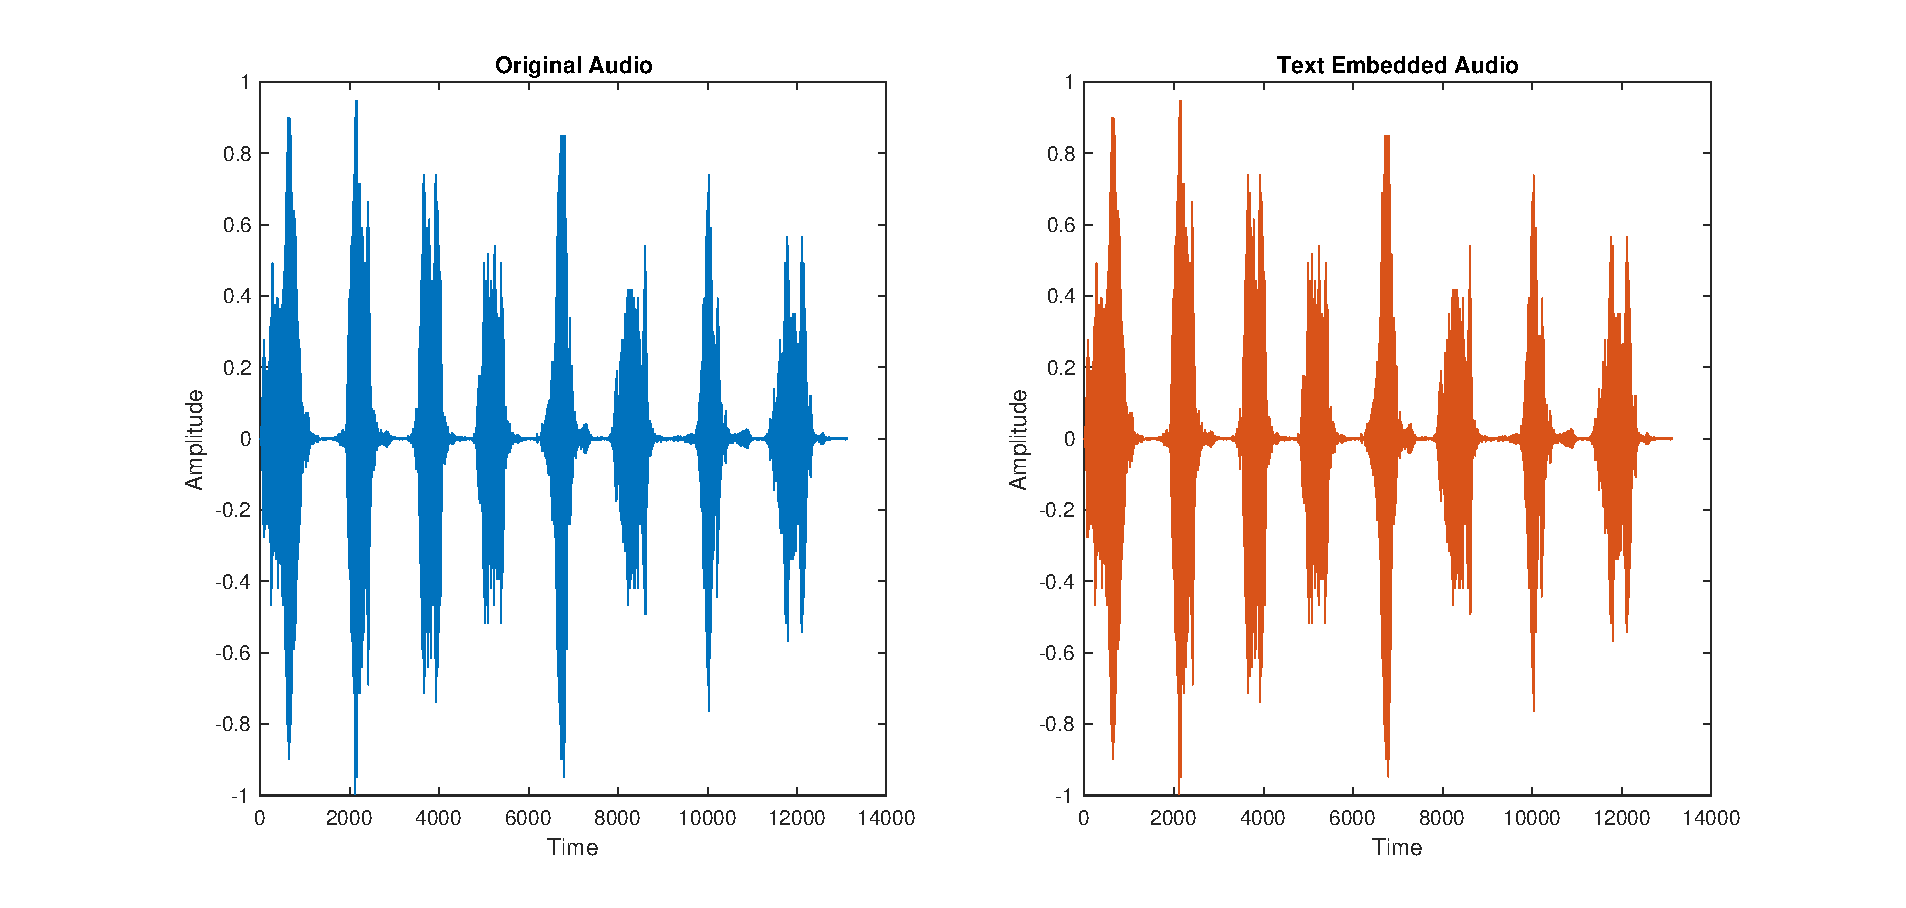
\includegraphics[scale=.32]{orig_vs_hidden.eps}
		\caption{Original Signal and Text Embedded signal side by side}
		\label{fig:versus}
	\end{figure}
	As can be seen from the Figure \ref{fig:versus}, there are not any imperceptible difference between original and manipulated difference. They are so similar to each so that even if one puts the plot on top of each other, it would be impossible to see the difference.
		\begin{figure}[h]
		\centering
		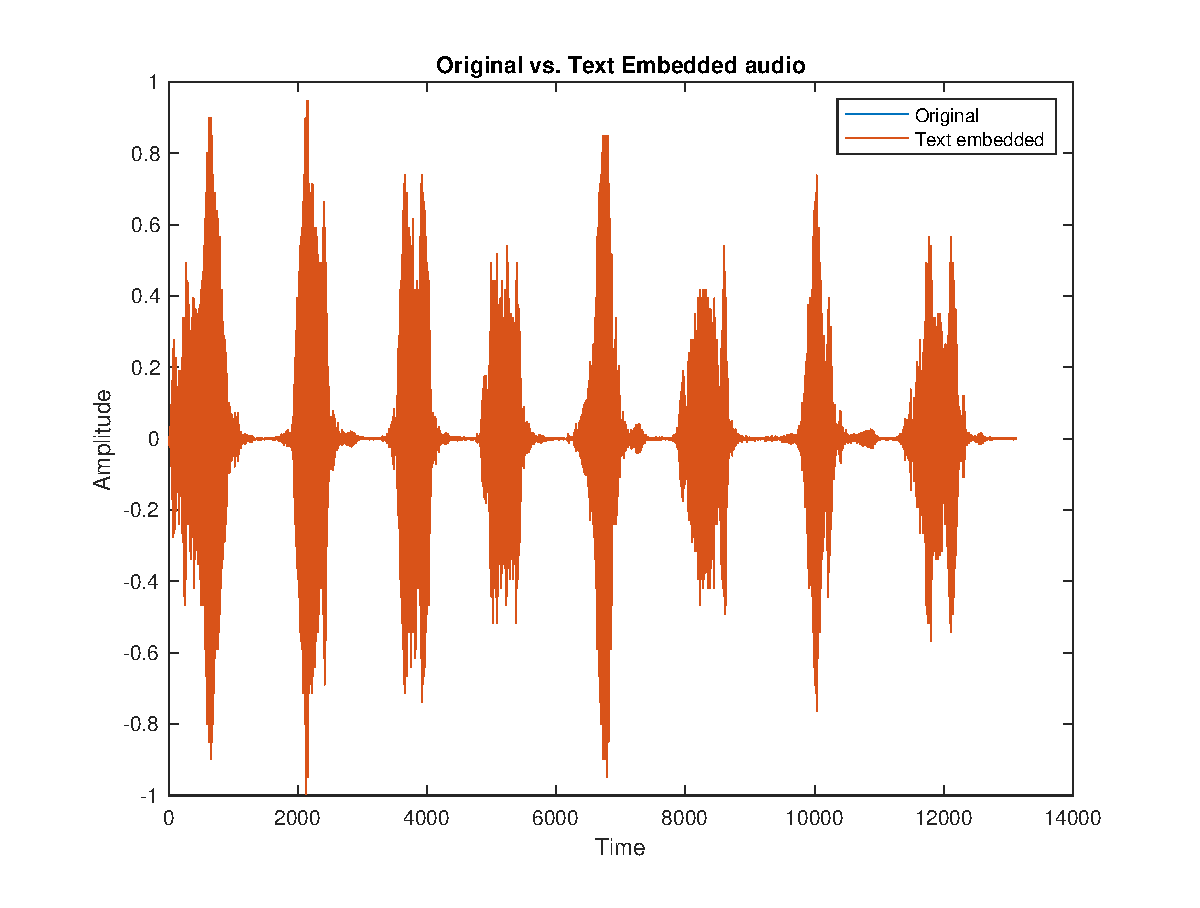
\includegraphics[scale=.5]{combined.eps}
		\caption{Original Signal and Text Embedded on top of each other}
		\label{fig:versus}
	\end{figure}

	This is what distinguishes LSB algorithm from other alternatives. It is impossible to notice any difference from the original signal if someone doesn't scrutinize the signal.  
	
	\section{Conclusion}
	This project covered the implementation of a steganography program from scratch, not using any external libraries or plugins but default functions of MATLAB. Through the project we learned about the audio signals in detail, how they are stored in computer memory and processed. Also, how the little changes on an audio signal doesn't make any noticeable difference to the original signal.
	
	\textit{Least Significant Bit Algorithm} is a basic level, relatively easy to understand and implement compared to other steganography algorithms. Each of the has trade-offs between security, robustness, discoverability etc. For this project, since it is not going to be used professionally in any area, we didn't had to dwell on those trade-offs. 
	
	
	\bibliographystyle{IEEEtran}
	\bibliography{references.bib}

\end{document}